\section{Experiment}
In this section, we conduct the following experiments to evaluate the prediction accuracy of the Mr. Prophet, and we compare the effectiveness of this new model with the What-IF~\cite{Herodotou2011Profiling} under a variety of input data and jobs.

\subsection{Experiment Setup}
We deploy a Hadoop cluster as the experimental environment to evaluate the Mr. Prophet. The Hadoop cluster with 16 machines is deployed, one of these machines is deployed as the master which runs the Resource Manager and the NameNode, and the other machines are deployed as the slave which runs the Node Manager and the Data Node.

Each machine in the cluster is with 16$\times$2.40GHz Processors and 50GB memory. The Hadoop version is 2.6.0, and the YARN(Yet Another Resource Negotiator)~\cite{Vavilapalli2013Apache} manages(allocate and deallocate) the resource of the Hadoop cluster. There are totally 240 cpu cores and 480 GB memory in the cluster, each machine in the cluster provides 16 cpu cores and 32 GB memory. Therefore, 240 map or reduce tasks can execute simultaneously, due to a map or reduce task requires 1 cpu core and 2 GB memory by default.

We use the HiBench~\cite{Huang2010The} as the benchmark suit, this benchmark suit contains 13 workloads, and we choose three typical workloads as our experimental workloads which are as follows. Wordcount(which counts the occurrence of each word in the input data.), Terasort(which sorts the input data) and the Pagerank(which is MapReduce implementation of Pagerank algorithm.).

\subsection{The Accuracy of the New Model}
To validate the prediction accuracy of the MR. Prophet, the MapReduce jobs(Wordcount, Terasort and Pagerank) are required to execute on the Hadoop cluster once, and meanwhile the LTrace extracts the statistics of the MapReduce jobs, which is the prerequisite for the prediction. Then the execution time of these jobs with various input data is predicted by the new model and What-IF respectively as follows.

To illustrate the effectiveness of the new model, we establish the following evaluation indicator.
\begin{small}
\begin{equation}
\begin{split}
I_{accu}=\frac{|T_{wf}-T_a|}{T_a} - \frac{|T_{new}-T_a|}{T_a}
\end{split}
\end{equation}
\end{small}

\emph{where the $I_{acct}$ is the indicator value which represents the improvement of the MR. Prophet's prediction accuracy relative to the What-IF, the $T_a$ represents the actual execution time of the MapReduce job, the $T_{wf}$ is the execution time predicted by the What-IF, and the $T_{new}$ is the execution time predicted by the MR. Prophet.}

As shown in the equation (6), the $\frac{|T_{wf}-T_a|}{T_a}$ is the relative error of the What-IF's prediction accuracy, and the $\frac{|T_{new}-T_a|}{T_a}$ is the relative error of the new model's prediction accuracy. The decrease of relative error illustrate that the prediction accuracy of the new model is higher than the What-If's, and the higher the $I_{accu}$, the better the effectiveness of the MR. Prophet relative to the What-If.

\begin{table}[h]
\caption{The Prediction Accuracy of the MapReduce job's execution time}
\label{tab:tpa}
\newcommand{\tabincell}[2]{\begin{tabular}{@{}#1@{}}#2\end{tabular}}
\begin{center}
\footnotesize
\begin{tabular}{|c|c|c|c|c|c|}
\hline
\tabincell{c}{\textbf{Job}\\ \textbf{Name}} & \tabincell{c}{\textbf{Input}\\\textbf{(GB)}} & \tabincell{c}{\textbf{Actual}\\\textbf{(sec)}} & \tabincell{c}{\textbf{Mr. Prophet}\\\textbf{(sec)}} & \tabincell{c}{\textbf{What-IF}\\\textbf{(sec)}} & \tabincell{c}{$\textbf{I}_{\textbf{accu}}$\\\textbf{(\%)}}\\
\hline
 wordcount & 2 & 70 & 67 & 75 & 3.0 \\
 \hline
 wordcount & 10 & 123 & 118 &  142 & 11.9 \\
 \hline
 wordcount & 30 & 301 & 292 &  339 & 10.0 \\
 \hline
 wordcount & 50 & 469 & 491 & 541 & 10.6 \\
 \hline
 wordcount & 80 & 742 & 772 & 850 & 10.5 \\
 \hline
 wordcount & 100 & 920 & 960 & 1082 & 13.2 \\
 \hline
 terasort & 30 & 119 & 112 & 132 & 5.0 \\
 \hline
 terasort & 50 & 142 & 130 & 162 & 5.6 \\
 \hline
 terasort & 100 & 305 & 292 & 336 & 5.9 \\
 \hline
 terasort & 200 & 1020 & 960 & 1150 & 6.8 \\
 \hline
 pagerank & 31 & 279 & 266 & 313 & 7.5 \\
 \hline
 pagerank & 51 & 350 & 337 & 385 & 6.5 \\
 \hline
 pagerank & 92 & 645 & 624 & 728 & 9.6 \\
 \hline
\end{tabular}
\end{center}
\end{table}
Table \ref{tab:tpa} orderly shows the job's actual execution time, the job's execution time respectively predicted by the MR. Prophet and What-IF, and the $I_{accu}$ which illustrates the enhancement of our MR. Prophet relative to the What-IF under the various size of input data. As shown in the Table \ref{tab:tpa}, all the $I_{accu}$ of various jobs under the different input data  are greater than 0, which illustrates that the prediction accuracy of the MR. Prophet is better than the What-IF to some extent. For the application Wordcount, when the size of the job's input data reaches the 10 GB, all the $I_{accu}$ are greater than 10\%, which shows that our MR. Prophet owns much stronger forecasting ability than the What-IF especially for the large input data. This is because when the size of input data is larger, there are more data the reduce task have to process, and then there are more data to shuffle, which is simultaneously processed by the multiple copy threads and merge threads, therefore there are much more overlap time between the copy and merge phases, which can be captured by the MR. Prophet. For the applications Terasort and Pagerank, all the $I_{accu}$ are less than 10\%, it is because these jobs have over 100 reduce tasks, and the data processed by each reduce task is relatively small amount. Despite all this, the prediction accuracy of our MR. Prophet is above 94\% for the Terasort and Pagerank. It is noteworthy that all the execution time predicted by the What-IF are greater than the actual execution time, which demonstrates that the executing procedure of Hadoop MapReduce job is extremely complex and it is not simply executed step by step. Therefore, it is necessary to find out the parallels between multiple different phases and quantify the overlap time of these parallel phases.

The execution of MapReduce job consists of the map tasks and reduce tasks, the prediction accuracy of the map and reduce tasks' execution time is shown as the follows.

\begin{table}[h]
\caption{The Prediction Accuracy of the Map Task's execution time }
\label{mapexe}
\newcommand{\tabincell}[2]{\begin{tabular}{@{}#1@{}}#2\end{tabular}}
\begin{center}
\footnotesize
\begin{tabular}{|c|c|c|c|c|c|}
\hline
\tabincell{c}{\textbf{Job}\\\textbf{Name}} & \tabincell{c}{\textbf{Input}\\\textbf{(GB)}} & \tabincell{c}{\textbf{Actual}\\\textbf{(sec)}} & \tabincell{c}{\textbf{Mr. Prophet}\\\textbf{(sec)}} & \tabincell{c}{\textbf{What-IF}\\\textbf{(sec)}} & \tabincell{c}{$\textbf{I}_{\textbf{accu}}$\\\textbf{(\%)}}\\
\hline
 wordcount & 2 & 53.8 & 54.7 & 61.8 & 13.2 \\
 \hline
 wordcount & 10 & 53.1 & 54.7 & 61.8 & 13.4 \\
 \hline
 wordcount & 30 & 52.3 & 54.7 & 61.8 & 13.6 \\
 \hline
 wordcount & 50 & 55.5 & 54.7 & 61.8 & 12.7 \\
 \hline
 wordcount & 80 & 54.4 & 54.7 & 61.8 & 13.1 \\
 \hline
 wordcount & 100 & 53.9 & 54.7 & 61.8 & 13.2 \\
 \hline
 terasort & 30 & 32.6 & 28.4 & 29.2 & N \\
 \hline
 terasort & 50 & 33.5 & 28.4 & 29.2 & N \\
 \hline
 terasort & 100 & 31.2 & 28.4 & 29.2 & N \\
 \hline
 terasort & 200 & 35.9 & 28.4 & 29.2 & N \\
 \hline
 pagerank & 31 & 81.8 & 76.2 & 84.2 & N \\
 \hline
 pagerank & 51 & 80.2 & 76.2 & 84.2 & N \\
 \hline
 pagerank & 92 & 82.4 & 76.2 & 84.2 & N \\
 \hline
\end{tabular}
\end{center}
\end{table}
Table \ref{mapexe} shows the map task's actual execution time, the map task's execution time respectively predicted by the MR. Prophet and What-IF, and the $I_{accu}$. The input data of the map task has nothing to do with the input data of the MapReduce job, one map task processes a block of the HDFS, and the size of each block is uniform 128 MB by default, which can be specified by the related configuration parameter. Therefore, for the each application, the execution time of all the map tasks predicted by the model is the same due to the same block size of the HDFS. As shown in the table \ref{mapexe} , for the application Wordcount, all the $I_{accu}$ are greater than 10\%, and the prediction accuracy of our MR. Prophet for the map task is above 96\%. However, for the Terasort and Pagerank, our MR. Prophet can't predict accurately the execution time of the map task, this is because there are extra disk I/O latency during the phase of merge, the map task needs to create a new file and merge the relevant data of all the spill files into this new file for each reduce task, there are over 200 reduce tasks for these two jobs and 16 map tasks running simultaneously on one machine, therefore the disk I/O is so busy ,due to the frequent creation and access to various small files, which increases the latency of the disk I/O request response. Unfortunately, our MR. Prophet can't capture this latency of disk I/O request response, and the What-IF also doesn't not have this ability. The executing speed of the map task is affected by the number of reduce task to some extent, and it is a valuable experience to tuning the performance of the MapReduce jobs.

\begin{table}[h]
\caption{The Prediction Accuracy of the Reduce Task's execution time }
\label{tab:reduce}
\newcommand{\tabincell}[2]{\begin{tabular}{@{}#1@{}}#2\end{tabular}}
\begin{center}
\footnotesize
\begin{tabular}{|c|c|c|c|c|c|}
\hline
 \tabincell{c}{\textbf{Job}\\\textbf{Name}} & \tabincell{c}{\textbf{Input}\\\textbf{(GB)}} & \tabincell{c}{\textbf{Actual}\\\textbf{(sec)}} & \tabincell{c}{\textbf{Mr. Prophet}\\\textbf{(sec)}} & \tabincell{c}{\textbf{What-IF}\\\textbf{(sec)}} & \tabincell{c}{$\textbf{I}_{\textbf{accu}}$\\\textbf{(\%)}}\\
\hline
 wordcount & 2 & 13.9 & 12.6 & 12.9 & N \\
 \hline
 wordcount & 10 & 66.5 & 63.5 & 76.6 & 10.7 \\
 \hline
 wordcount & 30 & 245.1 & 239.8 & 277.4 & 11.1 \\
 \hline
 wordcount & 50 & 408.4 & 436.7 & 509.7 & 17.6 \\
 \hline
 wordcount & 80 & 680.3 & 717.4 & 835.2 & 17.3 \\
 \hline
 wordcount & 100 & 863.0 & 905.9 & 1072.2 & 19.7 \\
 \hline
 terasort & 30 & 52.4 & 55.4 & 62.5 & 13.5 \\
 \hline
 terasort & 50 & 69.7 & 72.8 & 86.1 & 19.1 \\
 \hline
 terasort & 100 & 165.7 & 172.4 & 202.1 & 17.9 \\
 \hline
 terasort & 200 & 260.5 & 276.3 & 329.2 & 20.3 \\
 \hline
 pagerank & 31 & 108.2 & 112.1 & 128.2 & 14.8 \\
 \hline
 pagerank & 51 & 175.1 & 184.9 & 208.3 & 13.4 \\
 \hline
 pagerank & 92 & 302.7 & 319.5 & 371.3 & 17.1 \\
 \hline
\end{tabular}
\end{center}
\end{table}
Table \ref{tab:reduce} shows the reduce task's actual execution time, the reduce task's execution time respectively predicted by the MR. Prophet and the What-IF, and the $I_{accu}$. The input data of the reduce task has a positive correlation with the MapReduce job's input data when the number of reduce tasks is invariant, there are more map tasks when there are more input data processed by the MapReduce job, therefore there are more output data of all the map tasks to be processed by each reduce task.  As shown in the Table \ref{tab:reduce}, for the application Wordcount, our MR. Prophet doesn't show the stronger ability than the What-IF, when the size of input data is 2 GB, this is because that all the 16 map tasks simultaneously execute on one machine, and the map tasks' outputs to be process by the reduce task are small, therefore there is only one copy thread fetching the map tasks' outputs and not merge thread merging the data in the buffer into the disk. For these three application, when the size of input data is larger, the $I_{accu}$ is higher, which indicates our MR. Prophet has stronger predictive ability than the What-If, especially when the input data is large. This is because there are more map tasks' outputs to be simultaneously copied into the reduce task by multiple copy threads, and meanwhile the merge threads are started to merge the buffer data or the multiple disk files into the disk file. The overlap time between the copy and merge phases increases rapidly, when the input data is getting larger, therefore it is so necessary to quantify the overlap time, and the unfortunate reality is that the What-IF doesn't have the ability to capture these overlap time. These experiments shows that our MR. Prophet can make up for the defect of the What-IF.
\begin{figure}[htbp]
\centering
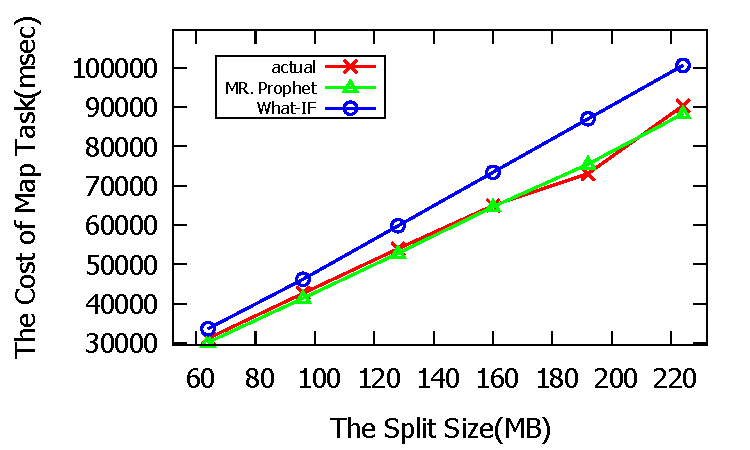
\includegraphics[height=5cm, width=8.5cm]{split}
\caption{The prediction for the map tasks with various split size}
\label{fig:map}
\end{figure}

To more fully illustrate the effectiveness of the MR. Prophet, we do an extra experiment to compare the prediction accuracy of the MR. Prophet and What-IF for the map tasks with various input data. We adjust the map task's input size by changing the configuration parameter dfs.block.size, and the parameter value is set from 64 to 224 MB. As shown in the Figure \ref{fig:map}, our MR. Prophet owns the strong ability to accurately predict the executing time of the map tasks with various input size. As expected, we can find that all the map tasks' execution time predicted by the What-IF are greater than the actual execution time, and the gap is more and more obvious when the input size increases. This is because the spill thread is started to spill the buffer data into the disk file when the size of buffer data reaches the spill threshold, and the main thread still executes the map function due to the remain free space of the buffer, hence there is overlap time between the map and spill phases. Unfortunately, the What-IF can not capture this overlap time between the map and spill phases. When the input size increases, there are more outputs of the map function to be spilled from the buffer into the disk file, which increases the overlap time accordingly. So what, our MR. Prophet holds the strong ability to capture these overlap time, which improves the predictive accuracy greatly.
